\documentclass[8pt,pdf,hyperref={unicode}]{beamer}

% \documentclass[aspectratio=43]{beamer}
% \documentclass[aspectratio=1610]{beamer}
% \documentclass[aspectratio=169]{beamer}

\usepackage{lmodern}
\usepackage[russian]{babel}
\usepackage{subcaption}

% подключаем кириллицу 
\usepackage[T2A]{fontenc}
\usepackage[utf8]{inputenc}

\usepackage{mathrsfs} % буква для обозначения ЭДС
\newcommand{\EDS}{\ensuremath{\mathscr{E}}} % новая команда \EDS для символа

% отключить клавиши навигации
\setbeamertemplate{navigation symbols}{}

% тема оформления
\usetheme{CambridgeUS}

% цветовая схема
\usecolortheme{Beaver}

\title{Теплопроводность}   
\author{Никитин Илья}
\date{\today}

\begin{document}

	\maketitle
	
	\begin{frame}
		\frametitle{План доклада}
		\begin{center}
			\begin{itemize}
				\item Введение и описание эксперимента
				\item Теоретические выкладки
				\item Обработка данных и осмысливание результата
				\item Выводы и мысли о возможном усовершенствовании установки
			\end{itemize}
		\end{center}
	\end{frame}
	\begin{frame}
		\frametitle{Введение}
		\framesubtitle{Уравнение теплопроводности}
		\begin{center}
			\begin{equation}
				\frac{\partial T}{\partial t} - a^2 \Delta T = f(\vec{r}, t)
			\end{equation}
			где $f$ -- функция тепловых источников, $a^2 = \frac{\lambda}{c_p \rho}$ -- коэффициент температуропроводности, $\lambda$ -- теплопроводность, $c_p$ -- изобарная удельная теплоемкость, $\rho$ -- плотность.
		\end{center}
	\end{frame}
	\begin{frame}
		\frametitle{Введение}
		\framesubtitle{Установка для изучения теплопроводности}
		\begin{center}
			\begin{figure}[h!]
				\centering
				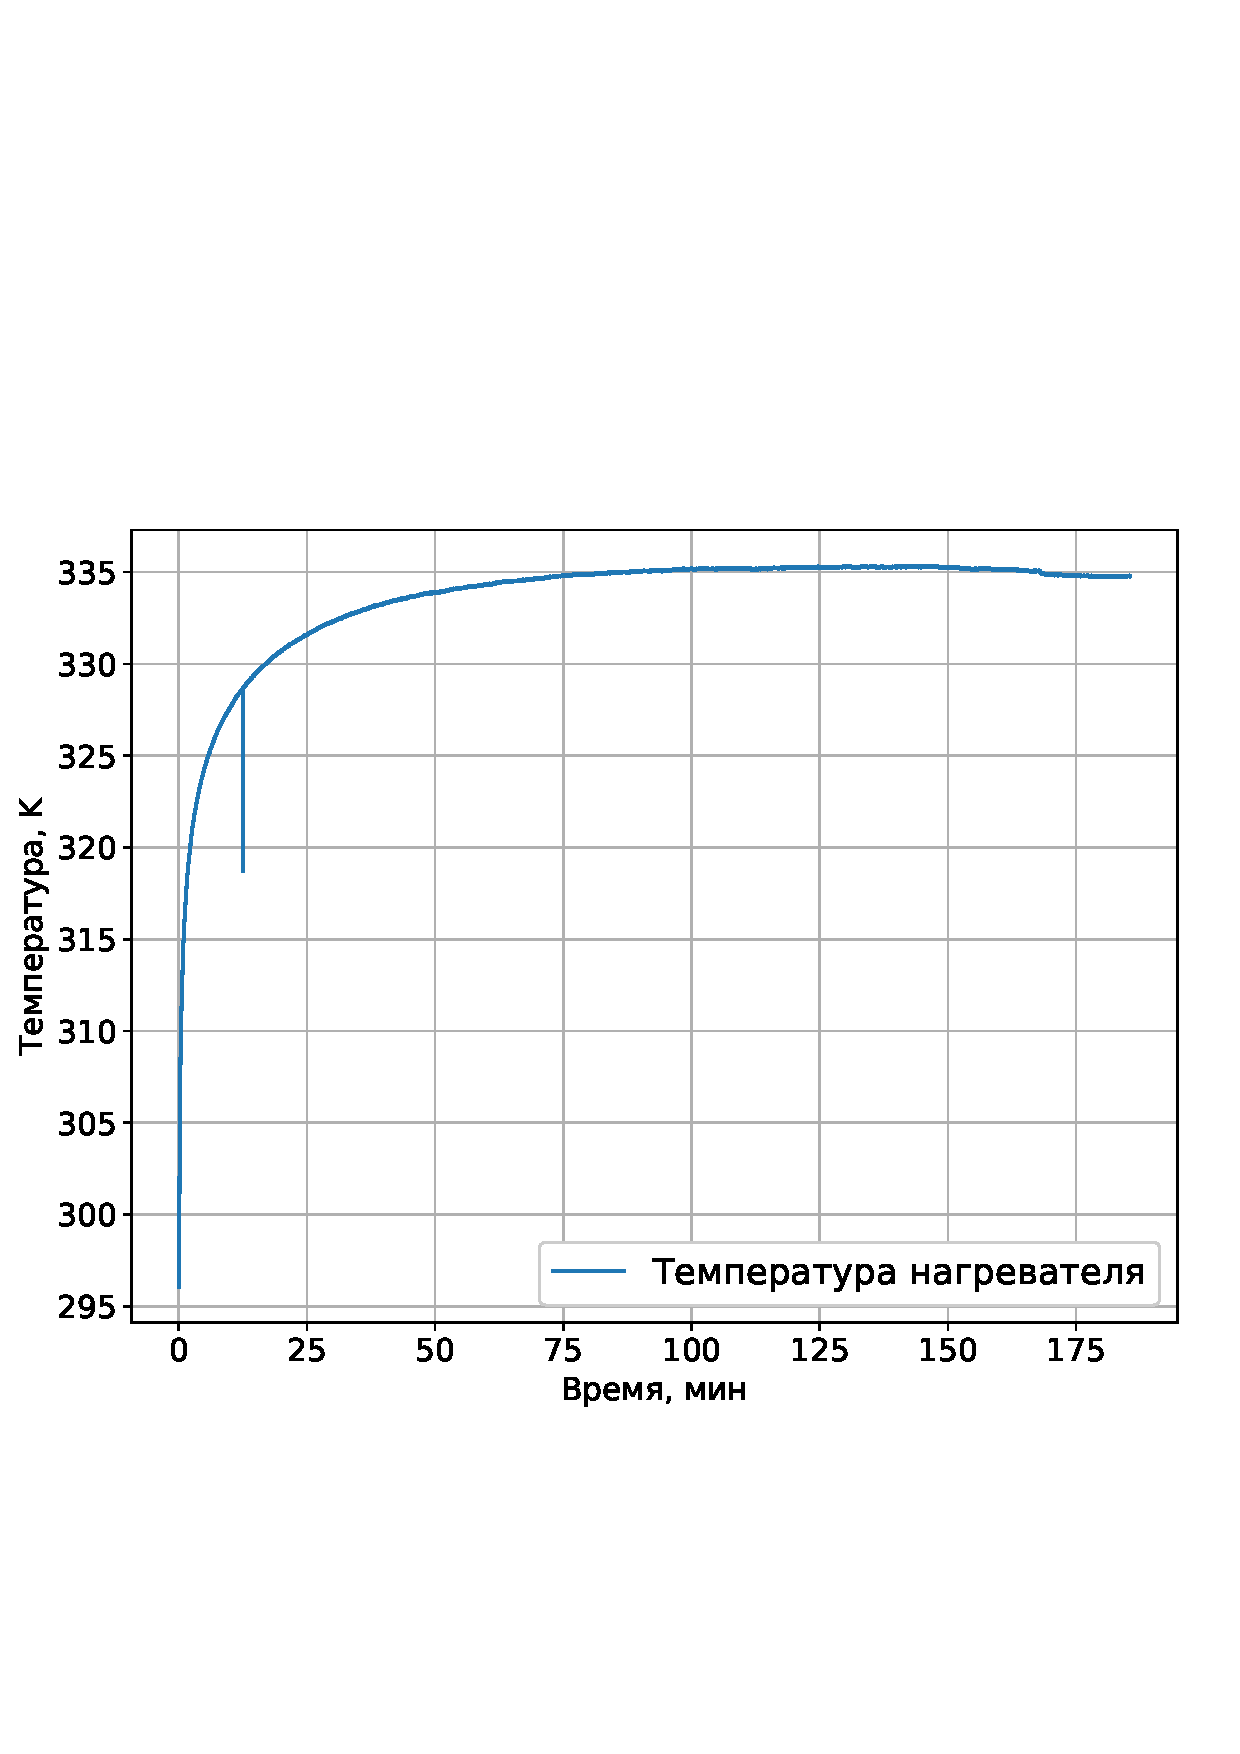
\includegraphics[width=.4\linewidth]{1.jpg}
				\caption{Сферическая колба с исследуемым материалом (манная крупа)}
				\label{fig1}
			\end{figure}	
		\end{center}
	\end{frame}
	\begin{frame}
		\frametitle{Введение}
		\framesubtitle{Установка для изучения теплопроводности}
		\begin{center}
			\begin{figure}[h!]
				\centering
				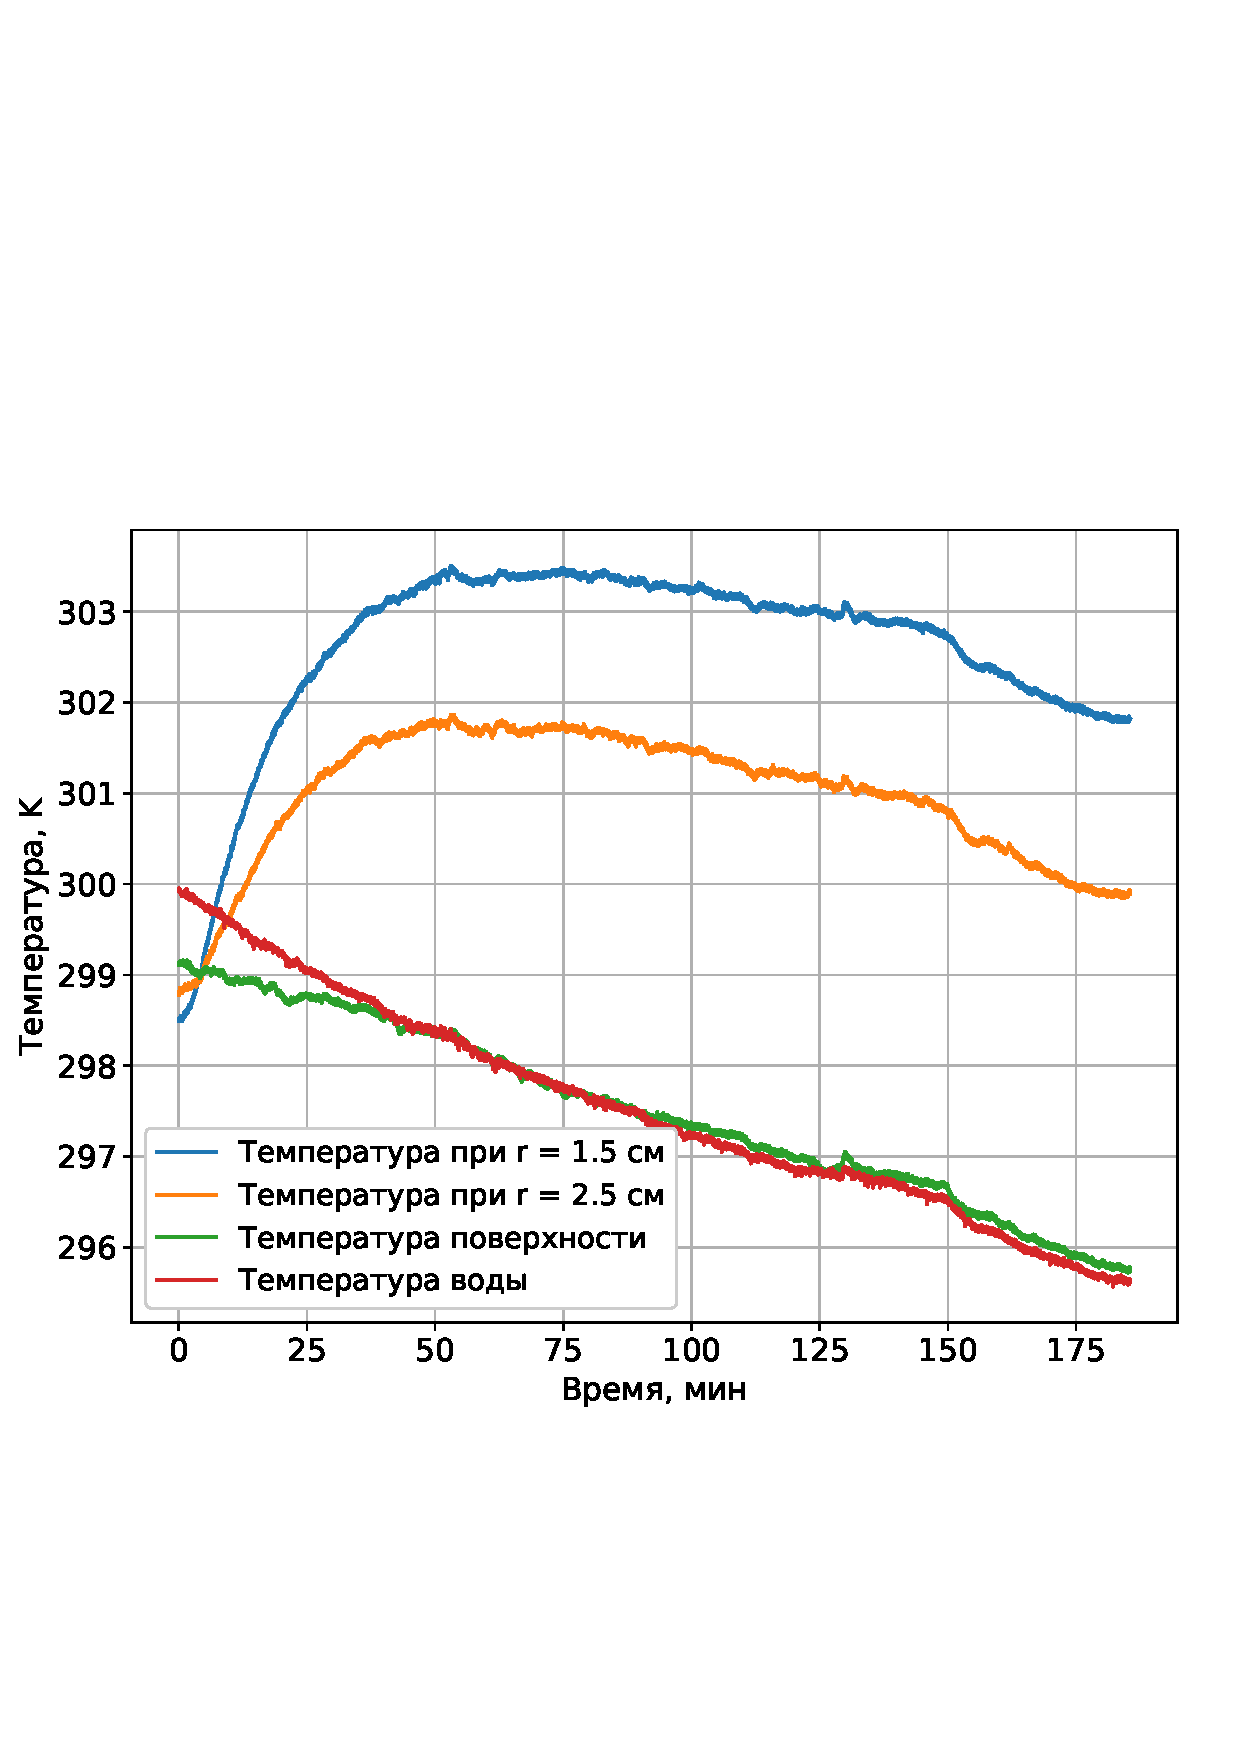
\includegraphics[width=.4\linewidth]{2.jpg}
				\caption{Нагреватель и несколько термопар}
				\label{fig2}
			\end{figure}
		\end{center}
	\end{frame}
	\begin{frame}
		\frametitle{Введение}
		\framesubtitle{Установка для изучения теплопроводности}
		\begin{center}
			\begin{figure}[h!]
				\centering
				\includegraphics[width=.4\linewidth]{3.jpg}
				\caption{Мультиметры Keysight, снимающие в автоматическом режиме показания с термопар}
				\label{fig3}
			\end{figure}
		\end{center}
	\end{frame}
	\begin{frame}
		\frametitle{Введение}
		\framesubtitle{Установка для изучения теплопроводности}
		\begin{center}
			\begin{figure}[h!]
				\centering
				\includegraphics[width=.7\linewidth]{4.jpg}
				\caption{Рабочий вид установки,	колба помещена в ведро с водой}
				\label{fig4}
			\end{figure}
		\end{center}
	\end{frame}
	\begin{frame}
		\frametitle{Введение}
		\framesubtitle{Установка для изучения теплопроводности}
		\begin{center}
			\begin{figure}[h!]
				\centering
				\includegraphics[width=.7\linewidth]{5.jpg}
				\caption{Программа на LabView, автоматически записывающая данные в реальном времени}
				\label{fig5}
			\end{figure}
		\end{center}
	\end{frame}
	\begin{frame}
		\frametitle{Теоретические выкладки}
		\framesubtitle{Уравнение теплопроводности в сферических координатах}
		\begin{center}
			В случае сферической симметрии удобно перейти к сферическим координатам. В таком случае $T = T(r)$:
			\begin{equation}
				\frac{\partial T}{\partial t} - a^2 (\frac{\partial^2 T}{\partial r^2} + \frac{2}{r} \frac{\partial T}{\partial r})  = f(r, t)
			\end{equation}
	
			Полагая $u = T \cdot r$:
			\begin{equation}
				\frac{\partial u}{\partial t} - a^2 \frac{\partial^2 u}{\partial r^2}  = f(r, t)
			\end{equation} 
		\end{center}
	\end{frame}
	\begin{frame}
		\frametitle{Теоретические выкладки}
		\framesubtitle{Стационарный случай}
		\begin{center}
			В случае, если температуры можно считать установившимися:
			\begin{equation}
			a^2 \frac{\partial^2 u}{\partial r^2}  = - f(r)
			\end{equation}
			
			В нашем случае при $r < r_0$: $f(r) = \frac{P}{V_0 c \rho}$, при $r > r_0$: $f(r) = 0$
		\end{center}
	\end{frame}
	\begin{frame}
		\frametitle{Теоретические выкладки}
		\framesubtitle{Результат решения дифференциального уравнения}
		\begin{center}
			Для области $r > r_0$:
			\begin{equation}
				T = T_0 + \frac{P r_0^2}{3 V_0 \lambda r}
			\end{equation}
			
			Отсюда:
			\begin{equation}
				\lambda = \frac{r P r_0^2}{3 V_0 (T - T_0)}
			\end{equation}
		\end{center}
	\end{frame}
	\begin{frame}
		\frametitle{Обработка данных}
		\framesubtitle{Температура нагревателя}
		\begin{center}
			\begin{figure}[h!]
				\centering
				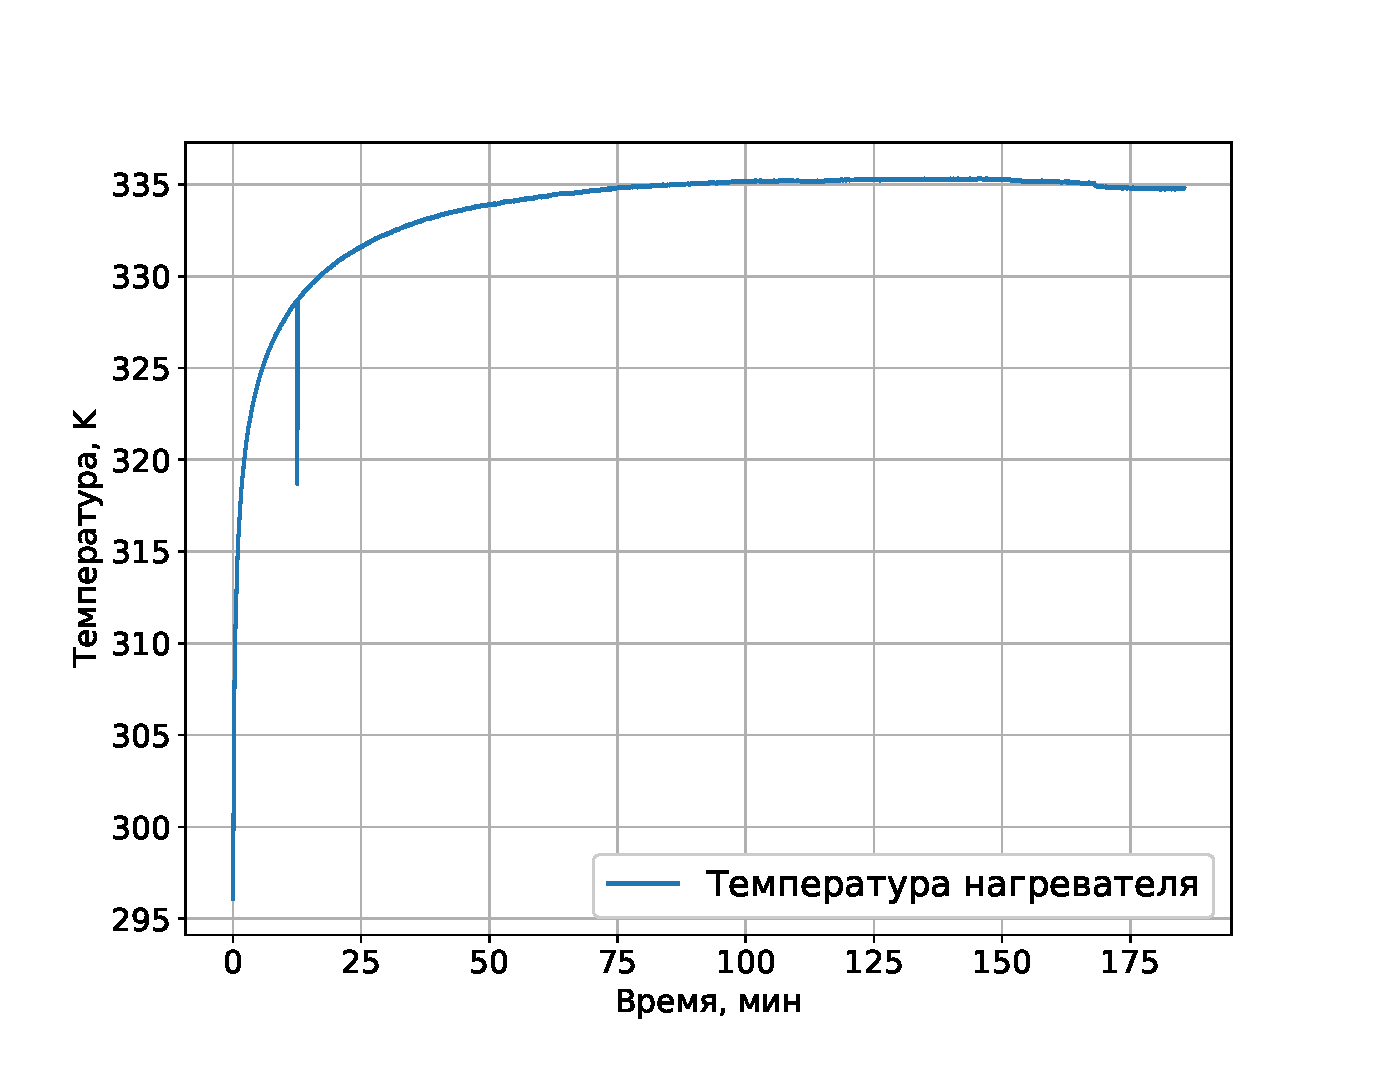
\includegraphics[width=0.7\linewidth]{1.eps}
				\caption{Температура нагревателя}
				\label{fig6}
			\end{figure}
		\end{center}
	\end{frame}
	\begin{frame}
		\frametitle{Обработка данных}
		\framesubtitle{Температуры внутри и вне шара}
		\begin{center}
			\begin{figure}[h!]
				\centering
				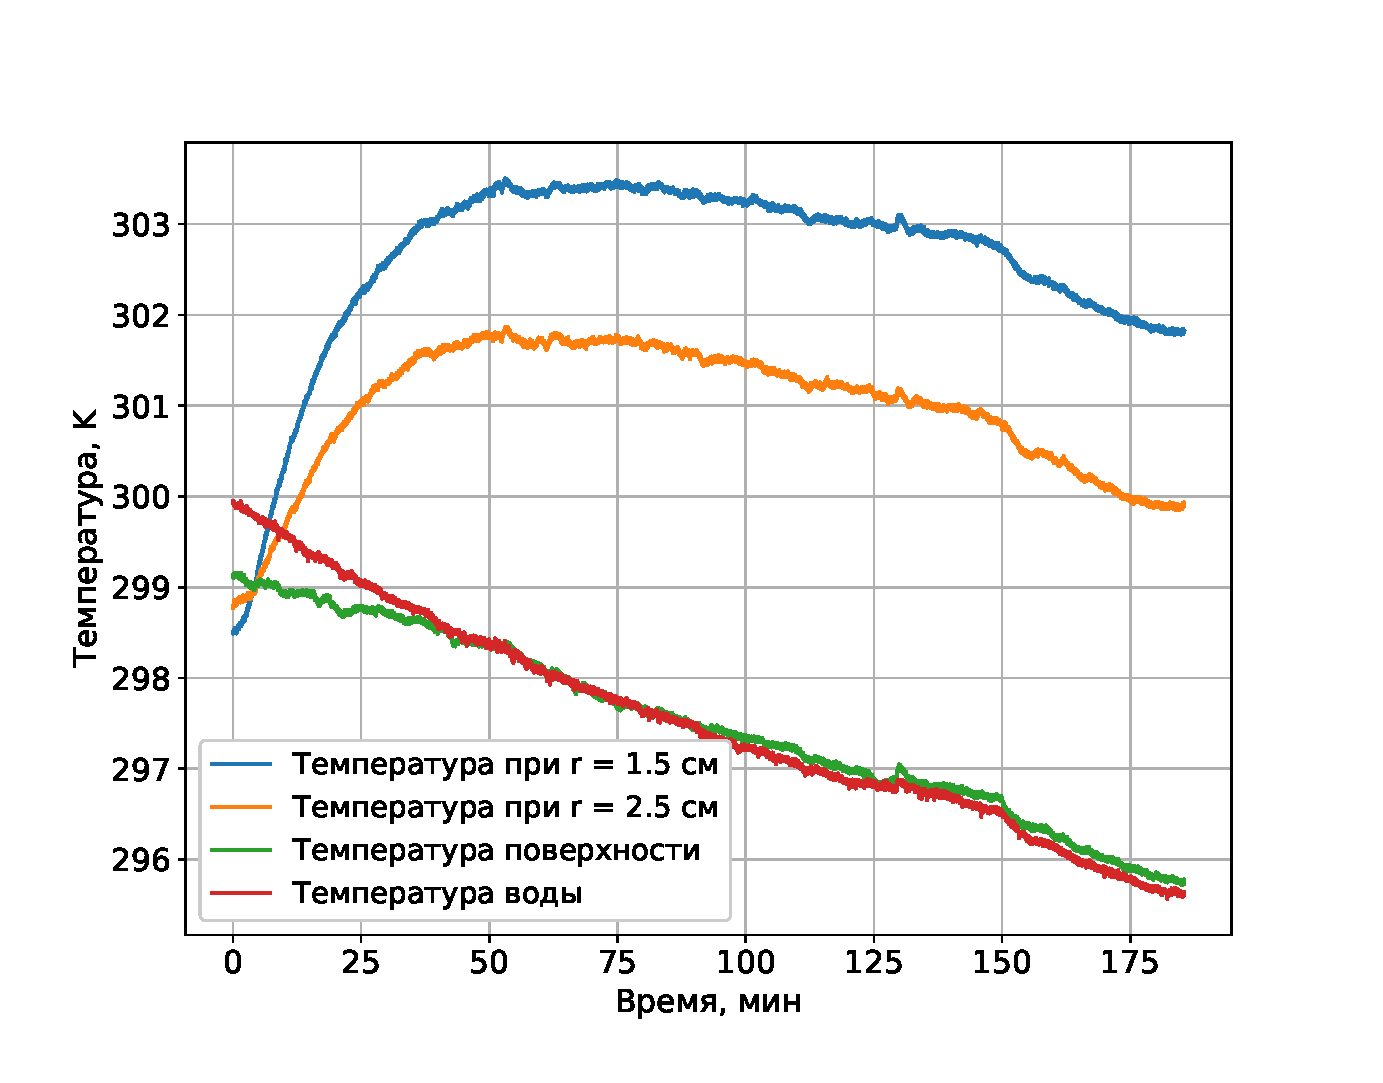
\includegraphics[width=0.7\linewidth]{2.eps}
				\caption{Температуры внутри и вне шара}
				\label{fig7}
			\end{figure}
		\end{center}
	\end{frame}
	\begin{frame}
		\frametitle{Обработка данных}
		\framesubtitle{Результат измерения теплопроводности}
		\begin{center}
		Считая, что изменения температуры со временем маленькие (в нулевом приближении стационарный режим) получаем:
			$\lambda = \frac{r P r_0^2}{3 V_0 (T - T_0)} \approx 0.26 \frac{\text{Вт}}{\text{м} \cdot \text{K}}$
		\end{center}
	\end{frame}
	\begin{frame}
		\frametitle{Выводы}
		\framesubtitle{Измерение температурных коэффициентов}
		\begin{center}
			\begin{itemize}
				\item Полученная теплопроводность манной крупы не сильно отличается от табличных значений для пшеничной крупы, что позволяет говорить о применимости такого метода измерения.
				\item В целом, можно было бы дополнить экспериментальную установку хорошим большим термостатом, для того, чтобы получить теплоемкость зерна, однако такого не оказалось на факультете.
			\end{itemize}		
		\end{center}
	\end{frame}
\end{document}